\section{Bidirectional transformation with TGGs}

\subsection{Possibilities with TGGs and Moflon}
For bidirectional transformations Tripple Graph Grammars (TGG) are used. These three graph based transformation contains a source, target and correspondence graph from which the transformation is derived. For more information about this transformation we refer you to work through Part IV of our handbook.
\newline
With this transformation there are many possible applications. In Fig.~\ref{Tgg_overview} is an overfiew of some posibilities which are treated in the handbook.

\begin{figure}[htbp]
	\centering
  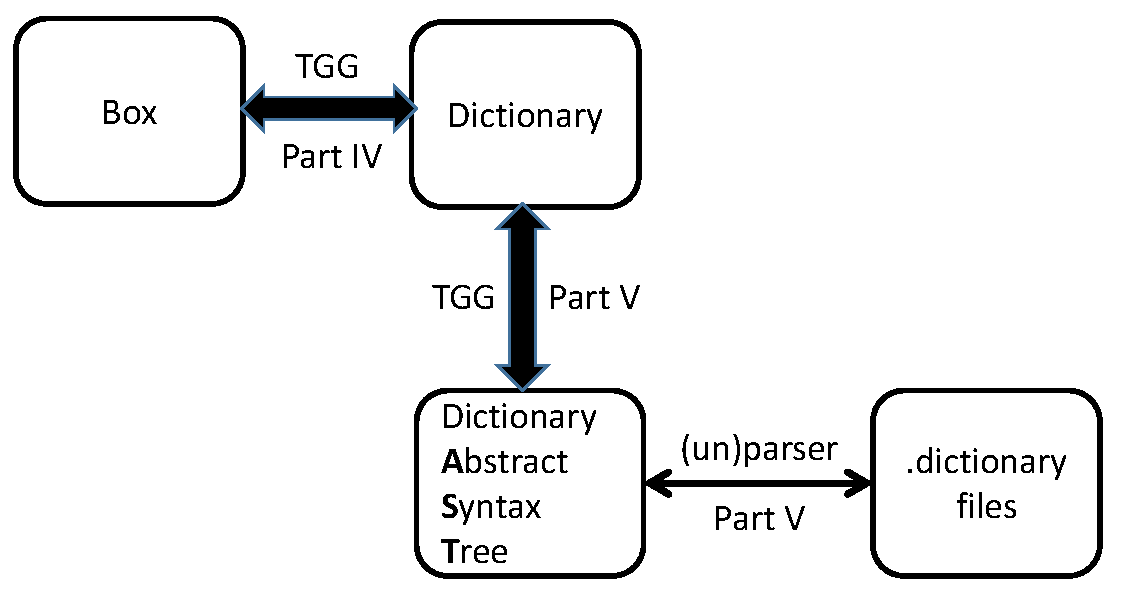
\includegraphics[width=0.9\textwidth]{TGG_overview.pdf}
	\caption{Overview of TGG usage} 
	\label{Tgg_overview} 
\end{figure}


With this transformation you are able to create bidirectional transformation between different metamodels, which is handled in Part IV, or even transform between an Abstract Syntax Tree and and an metamodel. After this you can also use an (un)parser to transform it into textfiles and wice versa. The latter is examined in Part V.


\subsection{Implementation of a TGG rule}
Now after you have a brief overfew over TGGs we will have a look at how you can use this in Moflon for creating bidirectional transformations.

\begin{itemize}
\item First set up your workspace. Like before check out the \texttt{Handbook Example (Final)} (Fig.~\ref{eclipse_checkout_final}).

\begin{figure}[htbp]
	\centering
  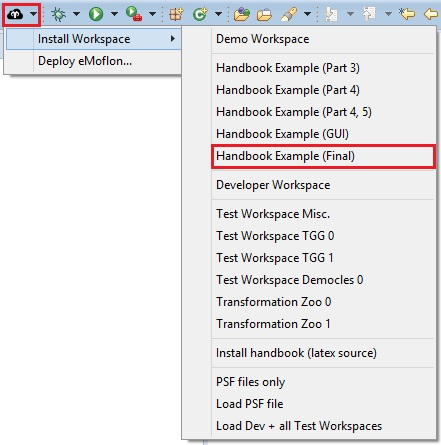
\includegraphics[width=0.8\textwidth]{eclipse_worcspace_final}
	\caption{Check out the Final Handbook Example} 
	\label{eclipse_checkout_final} 
\end{figure}

\item Next open the \texttt{Leitners\-Learning\-Box.eap} file in \texttt{Leitners\-Learning\-Box} (Fig.~\ref{eclipse_open_eap}).

\begin{figure}[htbp]
	\centering
  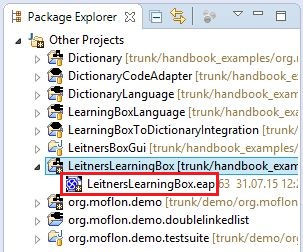
\includegraphics[width=0.5\textwidth]{eclipse_select_learningbox}
	\caption{Open \texttt{Leitners\-Learning\-Box.eap} file} 
	\label{eclipse_open_eap} 
\end{figure}

\item Because we transform here between two metamodels, we have two class diagrams, \texttt{LearningBoxLanguage} and \texttt{DictionaryLanguage}. For a better understanding open both like in Fig.~\ref{ea_select_classdiagrams}.

  \begin{figure}[htbp]
	\centering
  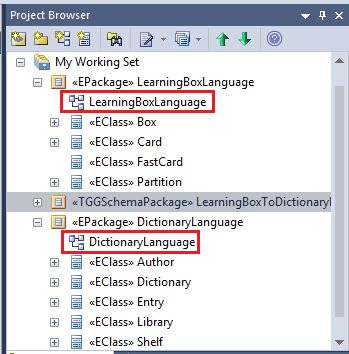
\includegraphics[width=0.55\textwidth]{ea_select_classdiagrams}
	\caption{Open the class diagrams \texttt{Learning\-Box\-Language} and \texttt{Dictionary\-Language}} 
	\label{ea_select_classdiagrams} 
\end{figure}

\end{itemize}

First have a look at \texttt{Learning\-Box\-Language} (Fig.~\ref{ea:classdiagram_LearningBoxLanguage}). Leitners Learning Box is a file card based learning system for vocabularies. It consists of a box with a certain number of partitions. In the partition are cards with vocabularies on it. How the cards are moved between the different partitions is for this tutorial not important. But if you want to know more about it work through Part II of our handbook.
\newline
In the classdiagram you can see that each element of the learning box is realized by an own class.

\begin{figure}[htbp]
	\centering
  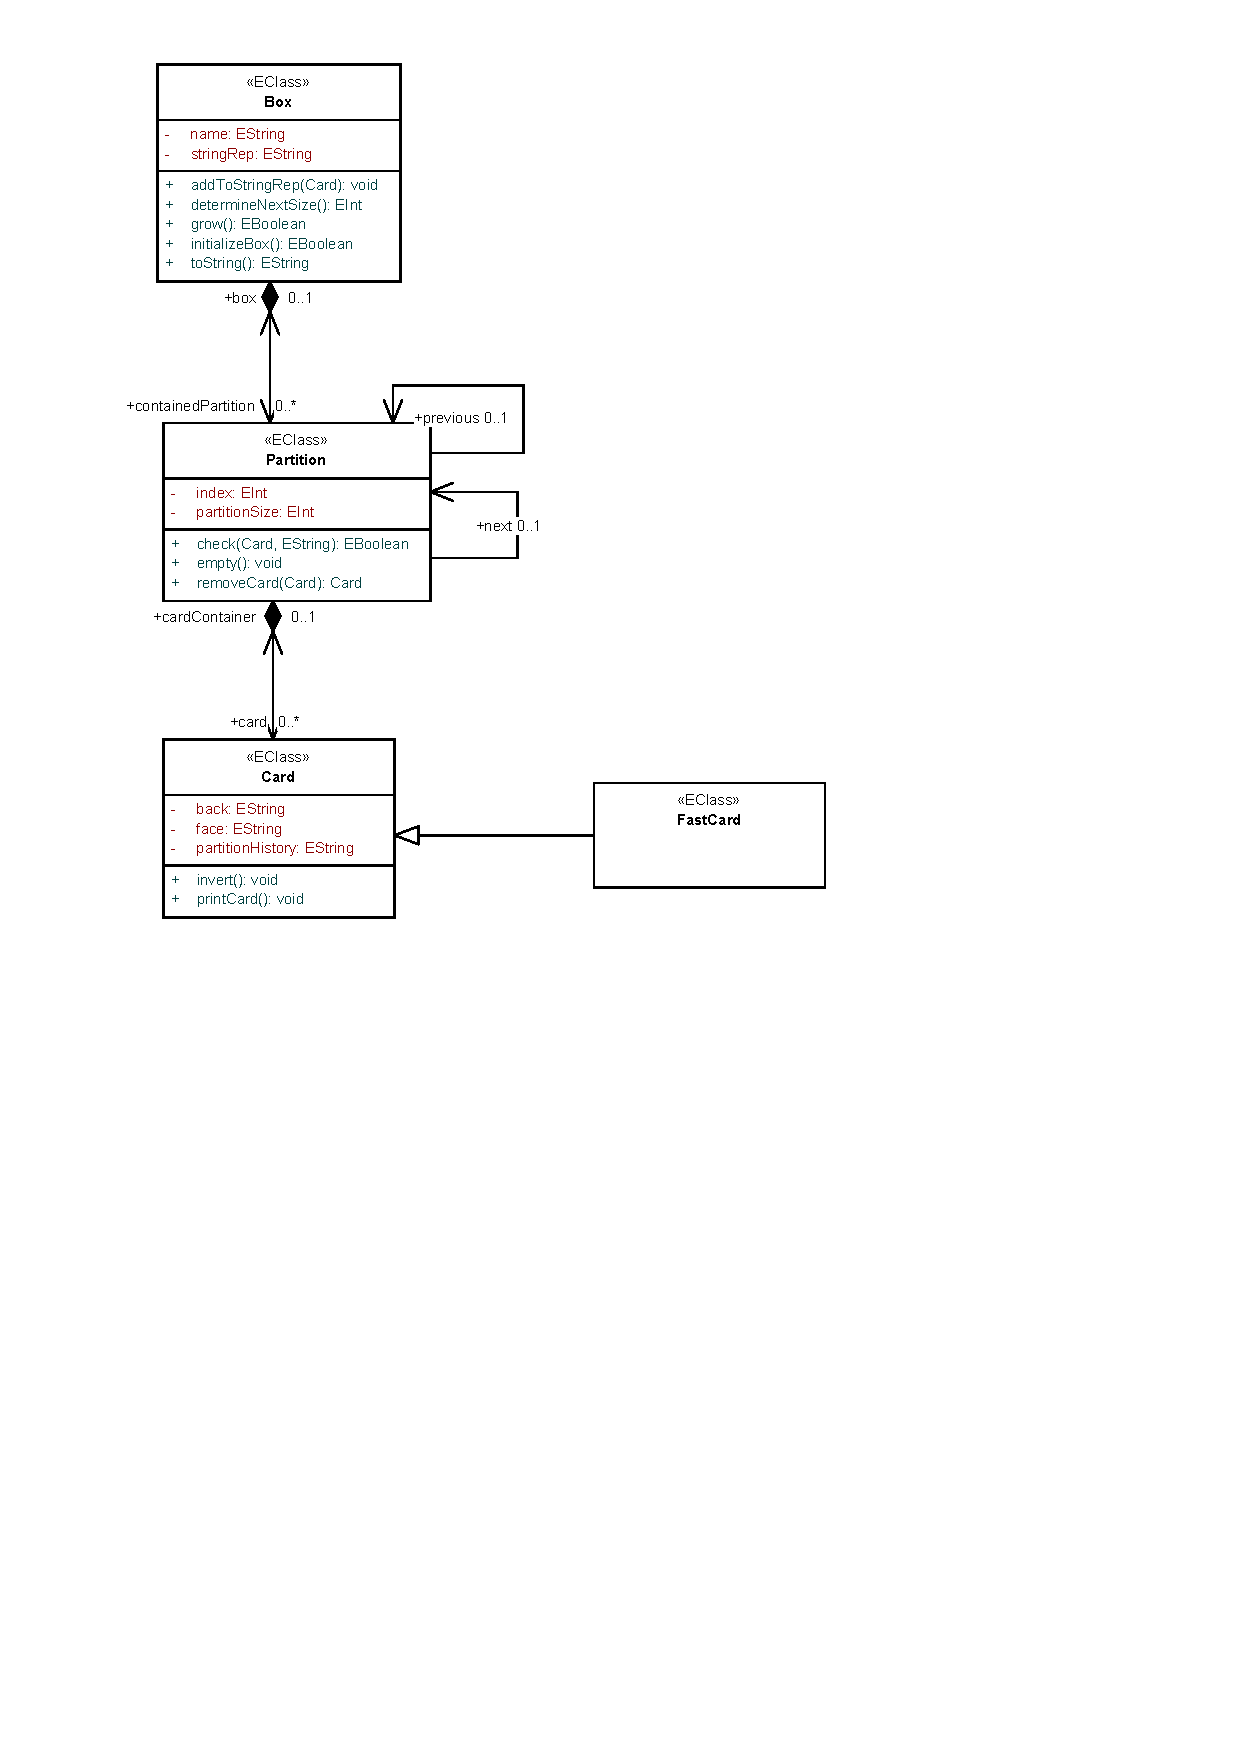
\includegraphics[width=1\textwidth]{LeitnersLearningBox_classdiagram}
	\caption{Classdiagram of \texttt{Learning\-Box\-Language}} 
	\label{ea:classdiagram_LearningBoxLanguage} 
\end{figure}

The other metamodel describes a library (Fig.~\ref{ea:classdiagram_DictionaryLanguage}). In a library you have different authors and shelfes, which contains the dictionary with some entries. this is how you imagine a library. Like as before every element of a library is here also a class.

\begin{figure}[htbp]
	\centering
  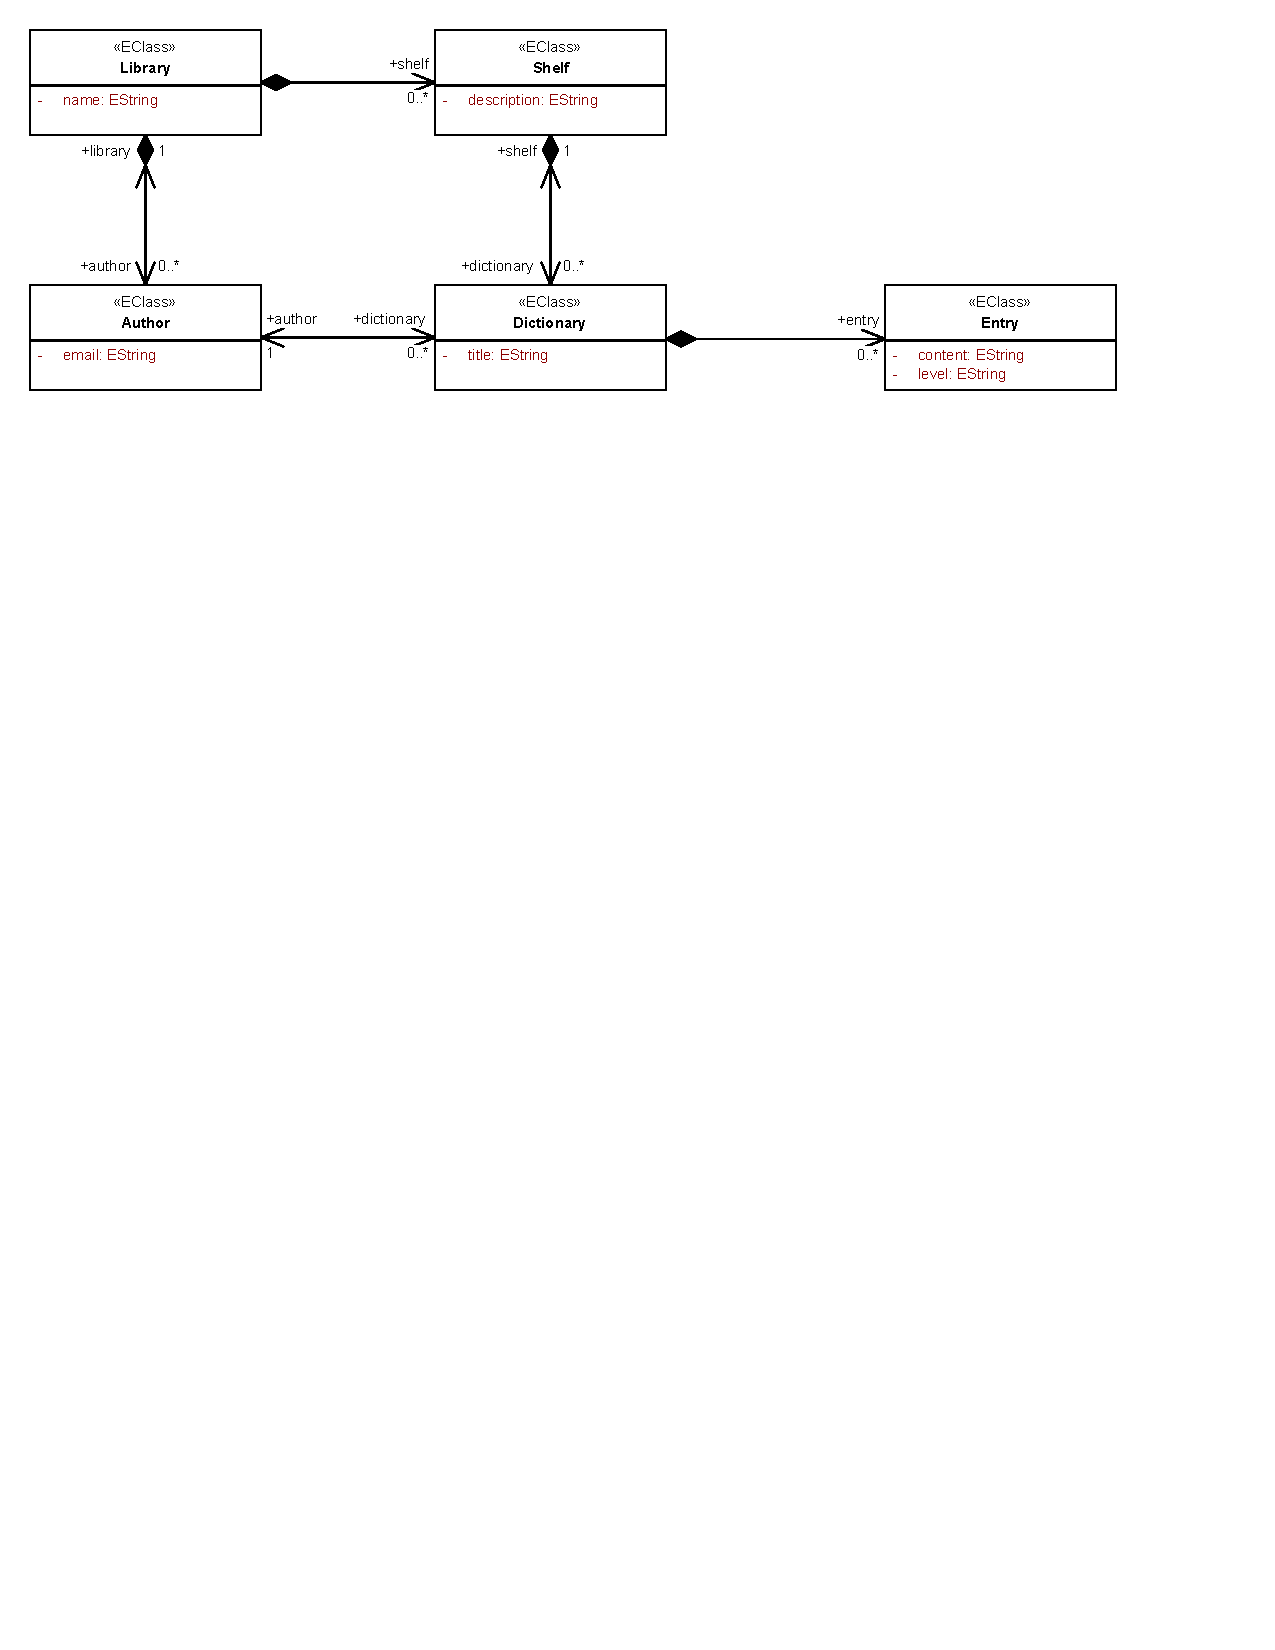
\includegraphics[width=1.2\textwidth]{Dictionary_classdiagram}
	\caption{Classdiagram of \texttt{Dictionary\-Language}} 
	\label{ea:classdiagram_DictionaryLanguage} 
\end{figure}

Now, after you know the two metamodels, we come to the transformation between them. For this we will examine one TGG rule as example.

\begin{itemize}

\item Open the \texttt{CardToEntryRule} in \texttt{Learning\-Box\-To\-Dictionary\-Integra\-tion/\-Rules} (Fig.~\ref{ea:openTGG_rule}).

\begin{figure}[htbp]
	\centering
  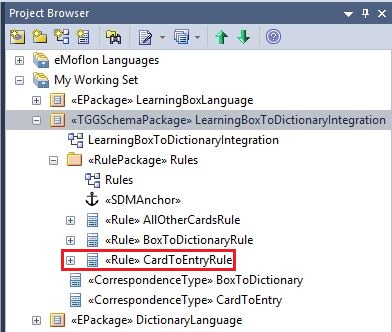
\includegraphics[width=0.6\textwidth]{ea_select_tgg_rule}
	\caption{Open the \texttt{CardToEntryRule}} 
	\label{ea:openTGG_rule} 
\end{figure}

\end{itemize}

\newpage % only for the layout
In Fig.~\ref{ea:TGG_rule} you see the \texttt{Card\-To\-Entry\-Rule}. In this rule we describe the transformation between card and entry. Like as at the SDM before black elements are here also context elements. In this case we have \texttt{box}, its correspondency \texttt{dictionary} and \texttt{partition0} as context elements. Green elements are the elements which are transformed in this rule, thus \texttt{card} and \texttt{entry}.
\newline
As mentioned before, TGG is a three graph based language. One source and target graph, which are left and right in Fig.~\ref{ea:TGG_rule}, and a correspondency graph in the middle. For the transformation between \texttt{card} and \texttt{entry} we have the corresponcy \texttt{cardToEntry}.
\newline
To set the attribute values we solving a \texttt{constraint satisfaction problem} (CSP). This is the black box at the bottom of the diagram. Here you have different possibilities to set or create the values. To know what you can do exactly and more details to the transformation with TGG we refer you to work through Part IV and V of our handbook.

\begin{figure}[htbp]
	\centering
  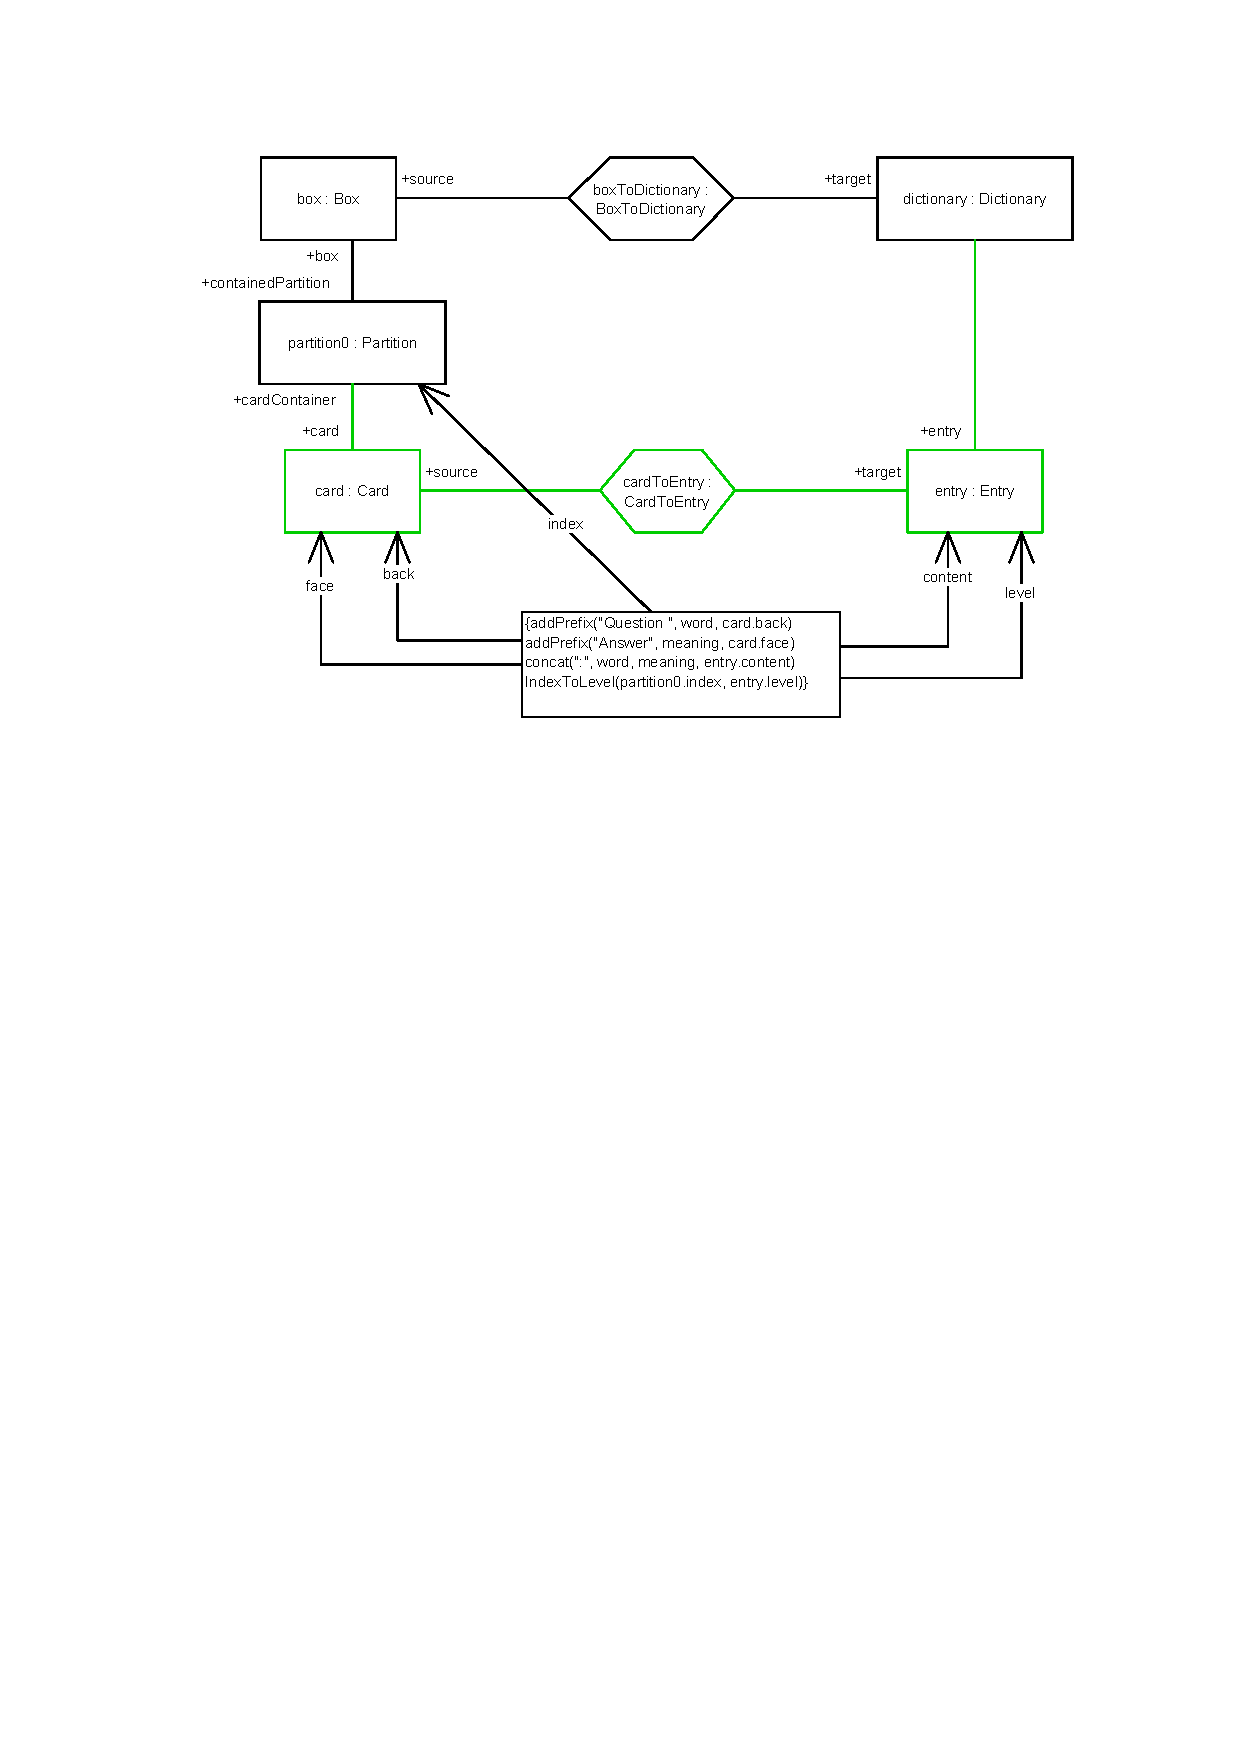
\includegraphics[width=1\textwidth]{TGG_rule}
	\caption{The TGG rule \texttt{CardToEntryRule}} 
	\label{ea:TGG_rule} 
\end{figure}